\section{Two Dimensional Graphics} \label{chap:two_dimensional_graphics}
OpenGL is a low-level graphics API.
It offers a set of functions to draw points, lines, and triangles.
It does not offer any functions to draw circles, ellipses, or other shapes.
That includes drawing text. 
Because of that adding the heads-up display (HUD) and the Menu to the game is not as simple as we would like it to be.
In this chapter, we describe how we draw 2d elements in our application.

\subsection{Textures} \label{sec:textures}
OpenGL does offer a way to draw images.
To draw an image you have to create a texture.
This texture is then passed to a shader.
You also have to create a VAO which contains vertices for a rectangle.
Each vertex has a position and a texture coordinate.
These texture coordinates are used to sample the texture using built-in shader functions.

Each image we want to draw can be represented by a texture.
For each image we want to draw, we can create a texture and pass it to the shader.
While this approach works, it is not very efficient.
Passing textures to the shader is a slow operation.
Because of that, we want to use as few textures as possible.
We can do that by combining multiple images into one.
We create Sprite Sheets which contain multiple images.
Each image in a sprite sheet (sprite) has a position and a size.
We can use this information to calculate the texture coordinates for each sprite.
We pass this information to the shader and use it to sample the correct part of the texture.
This way, we can pass a single texture to the shader and draw multiple images with it.

In our application, we have 2 sprite sheets.
The first one contains the images for the HUD.
This includes the inventory and all the items in it.
This sprite sheet is stored as a PNG file.
Sprite sheet with the inventory can be seen in \autoref{fig:inventory}.
It also has a JSON file which contains the position and size of each sprite which can be seen in \autoref{lst:inventory_sprite_sheet_json}.
The second sprite sheet contains the images of all letters and symbols used in the game.
This one is not stored in a file.
Instead, it is generated at runtime right after the program launches.
It uses SkiaSharp library to create a bitmap with all the ASCII characters.
This bitmap is then converted to a texture.
The position and size of each symbol is calculated using the font metrics.

These techniques are used to draw the HUD and the Menu.
Both of those are described in this chapter.

\begin{figure}[H]
    \centering
    \begin{minipage}{0.45\textwidth}
        \centering
        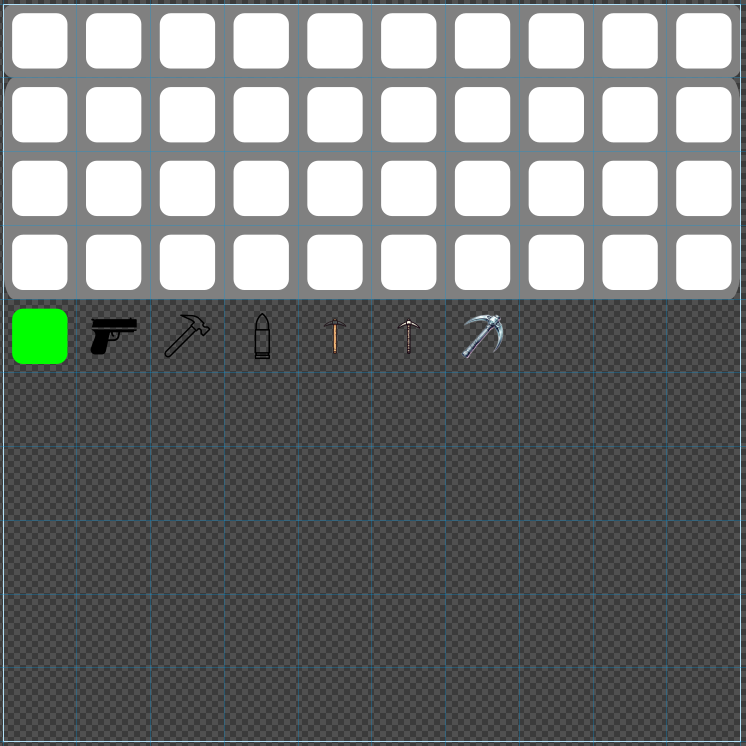
\includegraphics[width=0.8\textwidth]{chapters/system_architecture/sections/two_dimensional_graphics/resources/SpriteSheet.png}
        \caption{Inventory Sprite Sheet}
        \label{fig:inventory}
    \end{minipage}\hfill
    \begin{minipage}{0.45\textwidth}
    \begin{lstlisting}[language=json,firstline=1]
    {
        "width": 10,
        "height": 10,
        "items": [
            {
            "name": "hotbar",
            "x": 0,
            "y": 0,
            "width": 10,
            "height": 1
            },
        ]
    }
    \end{lstlisting}

    \caption{Inventory Sprite Sheet JSON}
    \label{lst:inventory_sprite_sheet_json}
    \end{minipage}
\end{figure}
\subsection{Heads Up Display} \label{sec:hud}
The HUD encapsulates all the 2d elements that are drawn on top of the 3d scene while the game is runnings.
This includes:
\begin{itemize}
    \item Crosshair
    \item FPS counter
    \item Player position
    \item Inventory
\end{itemize}

The Crosshair is a simple cross in the middle of the screen.
It is used to help the player aim.
It consists of 2 lines and does not use any textures.

The FPS counter is a simple text that shows the current frame rate.
It is drawn in the top right corner of the screen.
It uses the symbols texture.

The player position is a simple text that shows the current position of the player.
It is drawn in the top left corner of the screen.
It uses the symbols texture.

The inventory is a collection of images that represent the items the player has.
It is drawn at the bottom of the screen.
It uses both the items texture containing the HUD items and the texture containing the alphabet.
The images of the items are drawn first and then the text is drawn on top of them.
It is done in this order to optimize the performance by minimizing the number of times a texture is set to 2.

All the elements of the HUD have their own positions and sizes.
Each element is either placed in some position on the screen or is placed relative to some other element.
\subsection{Menu} \label{sec:menu}
Menu is a lot more complicated than the HUD which is described in \autoref{sec:hud}.
Because of that we decided to create a framework for creating menus.
This framework was heavily inspired by Flutter.
It uses the same concepts and terminology.
The overall idea is that everything is a widget.
A widget is a class that has a \texttt{Render} method as well as a \texttt{GetSize} method.
The \texttt{Render} method takes a context which includes information about the position and size on the screen that the widget can render to.
Some widgets also have children so the overall structure of the menu is a tree of widgets.

An example of a widget is shown in \autoref{fig:example_widget}.
This widget renders the main menu of the game.
The rendering logic of this widget can be seen in \autoref{fig:widget_logic}.
The idea is as follows.
The root widget calls the render method of it's child which is the \texttt{Background} widget.
The \texttt{Background} widget renders a background color.
Then the \texttt{Background} widget calls the render method of it's child which is the \texttt{Column} widget.
This widget renders it's children in a column but to do that it first needs to know the size of each of its children.
Based on that information it will call a render method of each child with the appropriate context.
Each child asks it's children for their size recursively until it reaches a leaf widget.
The process stops at the leaf and the render method is called on the children of the column widget.

This is a simplified version of the rendering logic as each widget has multiple options and rules that change how it or it's children are rendered.
For example, the \texttt{Column} widget has a \texttt{alignment} property which changes how the children are aligned.
The \texttt{Button} widget in the \autoref{fig:widget_logic} itself is a tree of widgets.

This approach of rendering the menu is very flexible and allows for a lot of customization.
It improves on the method used to render the HUD described in \autoref{sec:hud}.
This approach is not common in game development.
Usually menus are created by putting elements on the screen at specific positions. % TODO: cite something
In this part we believe that our approach is better than the traditional one and improves on approaches used in most popular game engines like Unity or Godot.

\begin{figure}[H]
    \centering
    \begin{minipage}{0.45\textwidth}
        \centering
        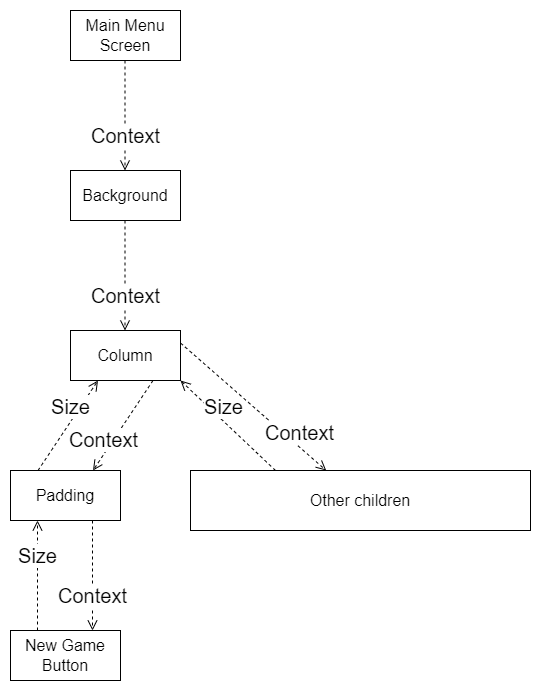
\includegraphics[width=0.8\textwidth]{chapters/system_architecture/sections/two_dimensional_graphics/resources/widget_logic.drawio.png}
        \caption{Widget rendering logic.}
        \label{fig:widget_logic}
    \end{minipage}\hfill
    \begin{minipage}{0.45\textwidth}
        \centering
        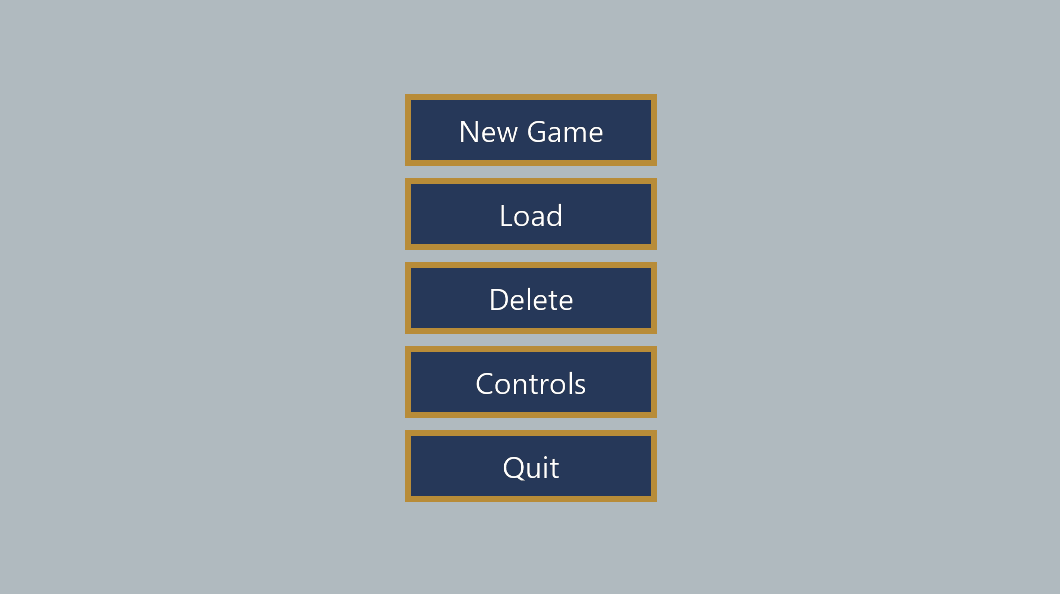
\includegraphics[width=0.8\textwidth]{chapters/system_architecture/sections/two_dimensional_graphics/resources/main-menu.png}
        \caption{Main menu.}
        \label{fig:example_widget}
    \end{minipage}
\end{figure}